% Capitolo 6 generato dalla bozza Markdown verificata.
\chapter{Testing e Mutation testing}\label{testing-e-mutation-testing}

\section{Obiettivi e metodologia della validazione}\label{obiettivi-e-metodologia-della-validazione}

La validazione sperimentale comprende sia i casi di test SCAS che hanno guidato lo sviluppo iniziale del sistema, sia ulteriori casi introdotti successivamente per ampliare e valutare le funzionalità supportate. Gli esperimenti considerano procedure relative a differenti funzioni della 5G Core Network, utilizzando come evidenza le informazioni ricavate dalle catture di traffico.

Sono inoltre previsti esperimenti di \emph{mutation testing} \cite{jia_harman_mutation_2011}, finalizzati a valutare la sensibilità del sistema ad alterazioni controllate dell'evidenza. La metodologia adottata e i relativi risultati sono approfonditi nella Sezione~\ref{mutation-testing}.

\section{Ambiente sperimentale e casi di test}\label{ambiente-sperimentale-e-casi-di-test}

Per la validazione sono stati utilizzati i seguenti ambienti e strumenti:

\begin{itemize}
\tightlist
\item
  Open5GS \cite{open5gs_docs}, implementazione open-source della 5G Core Network che fornisce le principali Network Functions previste dall'architettura 5G;
\item
  free5GC \cite{free5gc_docs}, implementazione open-source della 5G Core Network, utilizzabile per lo studio e la sperimentazione delle procedure e delle interazioni tra Network Functions;
\item
  ScasDK \cite{mancini_scasdk_2025}, piattaforma per l'esecuzione automatizzata di test di sicurezza SCAS, impiegata come riferimento sperimentale; alcuni suoi componenti sono stati adattati per le prove relative a NRF e UDM.
\end{itemize}

Il sistema proposto opera su catture di traffico già disponibili. L'esecuzione delle procedure SCAS e la generazione del traffico rimangono quindi distinte dalla verifica dell'esito e non rientrano tra le funzionalità della pipeline sviluppata, in accordo con il perimetro definito nella Sezione~\ref{scope-e-assunzioni}.

\Needspace{24\baselineskip}
I casi di test relativi alle funzioni NRF, UDM, AMF e UPF, definiti nelle rispettive specifiche SCAS \cite{3gpp_ts33518_2024,3gpp_ts33514_2021,3gpp_ts33512_2022,3gpp_ts33513_2023}, sono riepilogati nelle Tabelle~\ref{tab:open5gs_results} e~\ref{tab:free5gc_results}, organizzate in base all'implementazione della 5G Core Network da cui provengono le catture analizzate. Per ciascun caso vengono riportati il criterio di verifica applicato e il verdetto ottenuto.


\begin{center}
\begin{minipage}{\textwidth}
\centering

\begingroup
\small
\setlength{\tabcolsep}{5pt}
\renewcommand{\arraystretch}{1.3}

\begin{tabularx}{\linewidth}{|
    >{\raggedright\arraybackslash}p{0.31\linewidth}|
    >{\raggedright\arraybackslash}X|
    >{\centering\arraybackslash}p{0.19\linewidth}|}
\hline

\rowcolor{blue!7}
\textbf{Caso di test} &
\textbf{Criterio di verifica} &
\textbf{Verdetto} \\
\hline

NRF Discovery Authorization &
Risposta HTTP 403 &
FAIL \\
\hline

UDM Resynchronization &
Coerenza dei parametri di autenticazione &
PASS \\
\hline

UDM SUCI De-concealment &
SUPI restituito uguale al valore atteso &
PASS \\
\hline

AMF Sync Failure -- \mbox{Case A} &
Coerenza dei messaggi e \mbox{vincolo T3520} &
PASS \\
\hline

AMF Sync Failure -- \mbox{Case B} &
Coerenza dei messaggi e \mbox{vincolo T3520} &
PASS \\
\hline

UPF TEID Uniqueness &
Assenza di F-TEID duplicati &
PASS \\
\hline

AMF RES* -- Case A &
Gestione del fallimento di autenticazione &
PASS \\
\hline

AMF RES* -- Case B &
Gestione del fallimento di autenticazione &
\mbox{INCONCLUSIVE} \\
\hline

AMF RES* -- Case C &
Gestione del fallimento di autenticazione &
\mbox{INCONCLUSIVE} \\
\hline

AMF RES* -- Case D &
Gestione del fallimento di autenticazione &
\mbox{INCONCLUSIVE} \\
\hline

\end{tabularx}
\endgroup

\captionof{table}{Casi di test SCAS e verdetti ottenuti su Open5GS.}
\label{tab:open5gs_results}

\end{minipage}
\end{center}




\begin{center}
\begin{minipage}{\textwidth}
\centering

\begingroup
\small
\setlength{\tabcolsep}{5pt}
\renewcommand{\arraystretch}{1.3}

\begin{tabularx}{\linewidth}{|
    >{\raggedright\arraybackslash}p{0.31\linewidth}|
    >{\raggedright\arraybackslash}X|
    >{\centering\arraybackslash}p{0.19\linewidth}|}
\hline

\rowcolor{blue!7}
\textbf{Caso di test} &
\textbf{Criterio di verifica} &
\textbf{Verdetto} \\
\hline

AMF Sync Failure -- Case A &
Coerenza dei messaggi e vincolo T3520 &
PASS \\
\hline

AMF Sync Failure -- Case B &
Coerenza dei messaggi e vincolo T3520 &
PASS \\
\hline

AMF RES* -- Case A &
Gestione del fallimento di autenticazione &
PASS \\
\hline

AMF RES* -- Case B &
Gestione del fallimento di autenticazione &
PASS \\
\hline

AMF RES* -- Case C &
Gestione del fallimento di autenticazione &
PASS \\
\hline

AMF RES* -- Case D &
Gestione del fallimento di autenticazione &
PASS \\
\hline

\end{tabularx}
\endgroup

\captionof{table}{Casi di test SCAS e verdetti ottenuti su free5GC.}
\label{tab:free5gc_results}

\end{minipage}
\end{center}





I verdetti riportati rappresentano l'esito della verifica dei criteri dichiarati rispetto all'evidenza osservata. Un risultato \texttt{FAIL} non indica quindi necessariamente un malfunzionamento della pipeline, ma può corrispondere alla corretta rilevazione di un criterio non soddisfatto. È il caso del test NRF, nel quale la risposta osservata presenta uno status HTTP \texttt{200}, mentre la regola DSL richiede \texttt{403}.

\section{Valutazione delle capacità di verifica}\label{valutazione-delle-capacituxe0-di-verifica}

In questa sezione vengono approfonditi tre gruppi di casi di test, selezionati per esaminare il comportamento delle principali capacità di verifica implementate.

\subsection{AMF Synchronization Failure - Case B}\label{amf-synchronization-failure---case-b}

L'analisi di \texttt{AMF\ Synchronization\ Failure\ -\ Case\ B} coinvolge tre componenti del sistema: la selezione mediante \texttt{SEQUENCE}, la verifica statica sui campi degli eventi e la verifica temporale attraverso MonPoly.

Il caso riguarda la gestione di un fallimento di sincronizzazione durante la procedura di autenticazione 5G AKA. A seguito della ricezione di un'\texttt{Authentication\ Request}, l'UE segnala un \texttt{Authentication\ Failure} con causa di sincronizzazione e fornisce il parametro \texttt{AUTS} necessario alla risincronizzazione. L'AMF inoltra quindi le informazioni necessarie all'AUSF. Il timer NAS T3520, avviato dall'UE a seguito dell'invio dell'\texttt{Authentication\ Failure}, ha un valore di 15 secondi nelle condizioni ordinarie di accesso considerate \cite{3gpp_ts24501_2025}; tale intervallo è utilizzato come parametro di riferimento per il criterio temporale configurato nel test. Nel Case B, il criterio temporale verifica che, nell'intervallo configurato a partire dal fallimento di sincronizzazione, non venga osservata una nuova \texttt{Authentication\ Request} prima della risposta AUSF successiva alla richiesta di risincronizzazione.

\begin{figure}[!htbp]
\centering
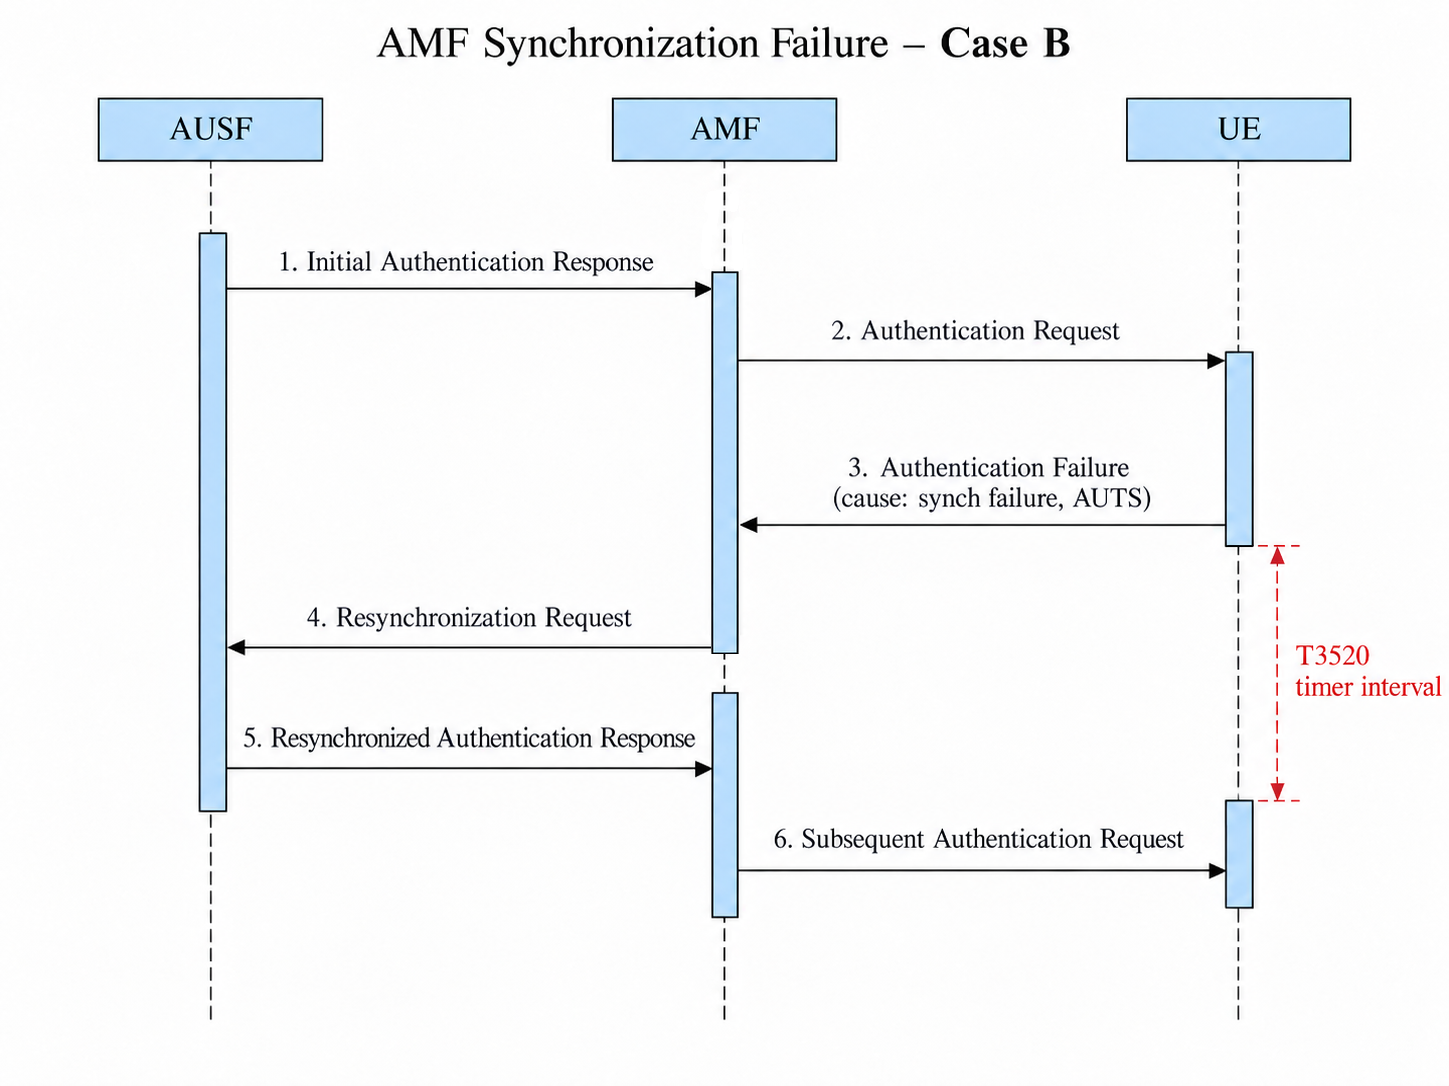
\includegraphics[width=0.94\textwidth,height=0.73\textheight,keepaspectratio]{figure/amf_sync_failure_case_b.png}
\caption{Scambio di messaggi nell'AMF Synchronization Failure, Case B, con vincolo temporale T3520.}
\label{fig:amf-sync-b}
\end{figure}

\Needspace{18\baselineskip}
La specifica DSL del caso descrive la successione degli eventi attesi e i criteri statici da valutare:

\par\noindent\begin{minipage}{\linewidth}
\begin{lstlisting}
SEQUENCE {
    ausf.authentication.response AS initial_vector
    nas.authentication_request AS initial_auth
    nas.authentication_failure AS sync_failure
    ausf.resynchronization.request AS resync
    ausf.authentication.response AS new_vector
    nas.authentication_request AS subsequent_auth_request
}

REQUIRE initial_auth.rand == initial_vector.rand
REQUIRE sync_failure.cause == 21
REQUIRE resync.auts == sync_failure.auts
REQUIRE resync.rand == initial_auth.rand
\end{lstlisting}
\end{minipage}\par

A questa si affianca la proprietà temporale MFOTL, che esclude la presenza di una nuova \texttt{Authentication\ Request} precedente alla risposta AUSF nell'intervallo configurato dopo il fallimento di sincronizzazione:

\par\noindent\begin{minipage}{\linewidth}
\begin{lstlisting}
MFOTL CASE B """
  SyncFailure()
  IMPLIES
  NOT (
      (NOT AusfAuthenticationResponse())
      UNTIL[0,{TIMER_MS}]
      AuthenticationRequest()
  )
"""
\end{lstlisting}
\end{minipage}\par

L'analisi delle catture provenienti da free5GC e Open5GS ha prodotto, in entrambi i casi, un unico match completo, associando agli alias dichiarati gli eventi individuati nel traffico. Le quattro verifiche statiche hanno restituito PASS per entrambe le implementazioni:

\begin{itemize}
\tightlist
\item
  corrispondenza del \texttt{RAND} tra risposta \texttt{AUSF} iniziale e l'Authentication Request;
\item
  presenza della causa \texttt{NAS\ 21} nell'Authentication Failure;
\item
  corrispondenza di \texttt{AUTS} tra l'Authentication Failure e la richiesta di risincronizzazione;
\item
  corrispondenza del \texttt{RAND} iniziale con quello utilizzato nella richiesta di risincronizzazione.
\end{itemize}

Anche la verifica temporale ha restituito PASS in entrambe le catture, sebbene siano stati osservati intervalli differenti tra i messaggi. In free5GC, l'Authentication Failure viene individuato al frame 358, mentre la successiva risposta AUSF e la nuova Authentication Request compaiono rispettivamente ai frame 604 e 606, circa 25 secondi dopo il fallimento di sincronizzazione. In Open5GS, gli stessi eventi vengono individuati ai frame 276, 432 e 434, con un intervallo di circa 11 secondi tra l'Authentication Failure e la nuova Authentication Request.

Nonostante la differenza negli intervalli osservati, in entrambe le catture la nuova Authentication Request segue la risposta AUSF. La verifica temporale restituisce quindi \texttt{PASS} per entrambe le implementazioni e, poiché anche i quattro criteri statici risultano soddisfatti, il verdetto complessivo è \texttt{PASS}. Il risultato mostra come la stessa specifica DSL e gli stessi componenti di verifica possano essere applicati a catture provenienti da implementazioni differenti, valutando sia la coerenza dei parametri scambiati sia le relazioni temporali tra gli eventi.

\subsection{UPF TEID Uniqueness}\label{upf-teid-uniqueness}

Il test \texttt{UPF\ TEID\ Uniqueness} impiega i costrutti \texttt{COLLECT} e \texttt{REQUIRE\ UNIQUE} per verificare l'unicità degli \texttt{F-TEID}, identificatori utilizzati per distinguere i tunnel GTP-U associati al traffico del piano utente. Durante l'instaurazione delle sessioni PFCP, l'UPF comunica tali identificatori attraverso i messaggi \texttt{PFCP\ Session\ Establishment\ Response}. La verifica considera gli \texttt{F-TEID} estratti dalle risposte osservate, controllando che non vengano riutilizzati tra eventi distinti.

La specifica DSL utilizzata è la seguente:

\par\noindent\begin{minipage}{\linewidth}
\begin{lstlisting}
COLLECT pfcp.session_establishment_response AS responses

REQUIRE UNIQUE responses.f_teids
\end{lstlisting}
\end{minipage}\par

La prima istruzione raccoglie tutti gli eventi corrispondenti al tipo semantico indicato, associandoli all'alias \texttt{responses}. La seconda applica il criterio di unicità ai valori \texttt{F-TEID} contenuti nella collezione, rappresentati come coppie strutturate \texttt{\{teid,\ ipv4\}}.

Nella cattura analizzata, il sistema ha individuato cinque risposte PFCP, corrispondenti ai frame 37, 38, 46, 47 e 48, dalle quali sono stati estratti complessivamente dieci F-TEID, due per ciascuna risposta. Pur condividendo lo stesso indirizzo IPv4, gli identificatori presentano valori TEID differenti; non essendo stata rilevata alcuna coppia \texttt{\{teid,\ ipv4\}} duplicata tra eventi distinti, il verificatore restituisce il verdetto complessivo \texttt{PASS}.



\subsection{AMF RES* Verification Failure - Cases A/B/C/D}\label{amf-res-verification-failure---cases-abcd}

Il test \texttt{AMF\ RES*\ Verification\ Failure} riguarda la gestione di un fallimento nella verifica della risposta di autenticazione \texttt{RES*} durante la procedura 5G AKA. Le quattro varianti considerate differiscono per il percorso di identificazione dell'UE e per l'origine del fallimento. L'identificazione può avvenire direttamente tramite SUCI oppure attraverso un'identificazione iniziale mediante GUTI, seguita da una richiesta d'identità; il fallimento può invece essere rilevato localmente dall'AMF oppure comunicato dall'AUSF.

Per rappresentare queste varianti mediante un'unica specifica DSL, vengono utilizzati i blocchi \texttt{OPTIONAL} per gli scambi di messaggi la cui presenza dipende dal percorso considerato e le regole \texttt{IF} per applicare i criteri di verifica corrispondenti alla configurazione del caso di test.

\Needspace{13\baselineskip}
Le combinazioni considerate sono riportate nella Tabella~\ref{tab:amf-res-varianti}.


\begin{center}
\begin{minipage}{\textwidth}
\centering

\begingroup
\small
\setlength{\tabcolsep}{5pt}
\renewcommand{\arraystretch}{1.25}

\begin{tabularx}{\textwidth}{|
    >{\centering\arraybackslash}m{0.08\textwidth}|
    >{\centering\arraybackslash}m{0.23\textwidth}|
    >{\centering\arraybackslash}m{0.21\textwidth}|
    >{\centering\arraybackslash}X|}
\hline
\rowcolor{blue!7}
\textbf{Caso} &
\textbf{Identificazione} &
\textbf{Origine del fallimento} &
\textbf{Eventi opzionali presenti} \\
\hline

A & SUCI diretto & AMF & Nessuno \\
\hline
B & GUTI $\rightarrow$ SUCI & AMF & Identity Request/Response \\
\hline
C & SUCI diretto & AUSF & Confirmation Request/Response \\
\hline
D & GUTI $\rightarrow$ SUCI & AUSF & Entrambi i gruppi \\
\hline

\end{tabularx}
\endgroup

\captionof{table}{Varianti del test AMF RES* Verification Failure}
\label{tab:amf-res-varianti}

\end{minipage}
\end{center}


La specifica DSL utilizza un'unica \texttt{SEQUENCE} contenente due blocchi \texttt{OPTIONAL}, rispettivamente dedicati agli scambi di identificazione e alla conferma dell'autenticazione con l'AUSF.


\par\noindent\begin{minipage}{\linewidth}
\begin{lstlisting}
SEQUENCE {
    nas.registration_request AS registration_request

    OPTIONAL {
        nas.identity_request AS identity_request
        nas.identity_response AS identity_response
    }

    ausf.authentication.response AS authentication_vector
    nas.authentication_request AS authentication_request
    nas.authentication_response AS authentication_response

    OPTIONAL {
        ausf.confirmation.request AS ausf_confirmation_request
        ausf.confirmation.response AS ausf_confirmation_response
    }

    nas.authentication_reject AS authentication_reject
}
\end{lstlisting}
\end{minipage}\par

\Needspace{23\baselineskip}
I criteri di verifica comprendono tre regole comuni, dedicate alla coerenza dei parametri \texttt{RAND} e \texttt{AUTN} e alla presenza dell'\texttt{Authentication\ Reject} finale. A queste si aggiungono le verifiche specifiche del percorso di identificazione dell'UE e dell'origine del fallimento, applicate in funzione della variante considerata.

\par\noindent\begin{minipage}{\linewidth}
\begin{lstlisting}
REQUIRE authentication_vector.rand == authentication_request.rand
REQUIRE authentication_vector.autn == authentication_request.autn
REQUIRE authentication_reject.present == true

IF case.identity_path == direct_suci {
    REQUIRE registration_request.identity_type == SUCI
}

IF case.identity_path == guti_then_suci {
    REQUIRE registration_request.identity_type == 5G_GUTI
    REQUIRE identity_request.requested_identity == SUCI
    REQUIRE identity_response.identity_type == SUCI
}

IF case.failure_source == local {
    REQUIRE hres_star.value != authentication_vector.hxres_star
}

IF case.failure_source == ausf {
    REQUIRE hres_star.value == authentication_vector.hxres_star
    REQUIRE authentication_response.res_star == ausf_confirmation_request.res_star
    REQUIRE ausf_confirmation_response.auth_result == AUTHENTICATION_FAILURE
}
\end{lstlisting}
\end{minipage}\par


Oltre ai binding prodotti dal matcher attraverso il riconoscimento degli eventi della sequenza, la specifica utilizza informazioni aggiuntive fornite al verificatore. In particolare, \texttt{case.identity\_path} e \texttt{case.failure\_source} sono \emph{binding di configurazione} che identificano rispettivamente il percorso di identificazione e l'origine del fallimento previsti dalla variante del test, mentre \texttt{hres\_star.value} è un \emph{binding derivato}, calcolato a partire dai parametri di autenticazione. Questi valori, pur non essendo ottenuti direttamente dal matcher, vengono integrati nel \texttt{BindingContext} insieme agli eventi selezionati, permettendo alla DSL di utilizzarli nelle regole di verifica.

L'analisi delle quattro catture free5GC ha prodotto un match completo per ciascuna variante, riconoscendo la presenza o l'assenza dei gruppi di eventi opzionali. I risultati delle verifiche sono riportati nella tabella seguente.




\begin{center}
\begin{minipage}{0.90\textwidth}
\centering
\begingroup
\small
\setlength{\tabcolsep}{5pt}
\renewcommand{\arraystretch}{1.18}

\begin{tabularx}{\linewidth}{|
    >{\centering\arraybackslash}X|
    >{\centering\arraybackslash}X|
    >{\centering\arraybackslash}X|
    >{\centering\arraybackslash}X|
    >{\centering\arraybackslash}X|}
\hline
\rowcolor{blue!7}
\textbf{Caso} &
\textbf{PASS} &
\textbf{SKIPPED} &
\textbf{Totale} &
\textbf{Verdetto} \\
\hline
A & 7  & 2 & 9  & PASS \\
\hline
B & 9  & 2 & 11 & PASS \\
\hline
C & 9  & 2 & 11 & PASS \\
\hline
D & 11 & 2 & 13 & PASS \\
\hline
\end{tabularx}

\endgroup
\captionof{table}{Risultati delle verifiche AMF RES* sulle catture free5GC. I conteggi includono anche i risultati aggregati dei blocchi IF.}
\label{tab:res-free5gc-details}
\end{minipage}
\end{center}




La differenza nel numero di criteri riportati dipende dalle verifiche applicabili a ciascuna variante. Tutti i casi condividono tre regole \texttt{REQUIRE} iniziali e quattro condizioni \texttt{IF}, ma il numero di regole interne eseguite varia in funzione del percorso osservato. Nel Case A, ad esempio, l'identificazione diretta tramite
\texttt{SUCI} e il fallimento locale richiedono una verifica
aggiuntiva ciascuno, mentre nel Case D il percorso
\mbox{\texttt{GUTI} $\rightarrow$ \texttt{SUCI}} e il fallimento
comunicato dall'AUSF comportano tre verifiche aggiuntive
per ciascuno dei due aspetti.





\paragraph{Confronto con le catture Open5GS.}
Una seconda verifica è stata eseguita su quattro catture Open5GS riferite alle stesse varianti RES*, applicando la medesima DSL e il verificatore comune. I risultati sono riportati nella Tabella~\ref{tab:res-open5gs}.

\begin{center}
\begin{minipage}{0.93\textwidth}
\centering
\begingroup
\small
\setlength{\tabcolsep}{4pt}
\renewcommand{\arraystretch}{1.18}
\begin{tabularx}{\linewidth}{|>{\centering\arraybackslash}p{0.08\linewidth}|>{\raggedright\arraybackslash}X|>{\centering\arraybackslash}p{0.27\linewidth}|}
\hline
\rowcolor{blue!7}
\textbf{Caso} & \textbf{Evidenza selezionata} & \textbf{Verdetto} \\
\hline
A & Match completo e criteri statici soddisfatti & PASS \\
\hline
B & Match completo; assenti i binding per Identity Request/Response & INCONCLUSIVE \\
\hline
C & Nessun match completo & INCONCLUSIVE \\
\hline
D & Nessun match completo & INCONCLUSIVE \\
\hline
\end{tabularx}
\endgroup
\captionof{table}{Verifica delle varianti AMF RES* su catture Open5GS.}
\label{tab:res-open5gs}
\end{minipage}
\end{center}


Per comprendere i risultati \texttt{INCONCLUSIVE} ottenuti nei Case B, C e D, è necessario distinguere le evidenze individuate durante la selezione. Nel Case B, il matcher riconosce una sequenza completa, associando agli eventi principali della procedura i frame 617, 624, 626, 627 e 628; tuttavia, gli alias \texttt{identity\_request} e \texttt{identity\_response}, appartenenti al blocco \texttt{OPTIONAL} dedicato all'identificazione, rimangono privi di un evento associato. Poiché tali binding sono richiesti dai criteri condizionali applicabili al percorso \mbox{\texttt{GUTI} $\rightarrow$ \texttt{SUCI}}, la verifica non può essere completata. Nei Case C e D, invece, il matcher non individua alcuna sequenza completa, impedendo già nella fase di selezione l'acquisizione delle evidenze necessarie per procedere alla verifica statica.

Questi risultati evidenziano due situazioni distinte. Nel Case B, il riconoscimento completo del pattern non garantisce la disponibilità di tutti i binding richiesti dai criteri applicabili, mentre nei Case C e D l'assenza di un match completo impedisce di avviare la verifica.


\section{Mutation testing}\label{mutation-testing}

Le mutazioni sono state introdotte nelle catture originali mediante procedure predisposte in funzione dei criteri definiti nelle rispettive specifiche DSL. Tali procedure appartengono all'infrastruttura sperimentale e operano sulle evidenze osservate, senza modificare l'interpretazione delle regole o la logica del verificatore.

\Needspace{15\baselineskip}
Le catture originali e quelle modificate vengono elaborate attraverso gli stessi meccanismi di selezione e verifica, così da confrontare i verdetti ottenuti e valutare la risposta del sistema alle alterazioni introdotte. La Tabella~\ref{tab:mutation-testing} riporta, per ciascuno scenario, la modifica effettuata e i risultati ottenuti prima e dopo la mutazione.

\begingroup
\footnotesize
\setlength{\tabcolsep}{3pt}
\renewcommand{\arraystretch}{1.25}

\begin{longtable}{|
    >{\raggedright\arraybackslash}p{0.23\textwidth}|
    >{\raggedright\arraybackslash}p{0.37\textwidth}|
    >{\centering\arraybackslash}p{0.12\textwidth}|
    >{\centering\arraybackslash}p{0.19\textwidth}|}

\hline
\rowcolor{blue!7}
\textbf{Caso di test} &
\textbf{Alterazione introdotta} &
\textbf{Baseline} &
\textbf{Mutato} \\
\hline
\endfirsthead

\hline
\rowcolor{blue!7}
\textbf{Caso di test} &
\textbf{Alterazione introdotta} &
\textbf{Baseline} &
\textbf{Mutato} \\
\hline
\endhead

NRF Discovery Authorization &
Status HTTP da 200 a 403 &
FAIL & PASS \\
\hline

UDM Resynchronization &
Alterazione del parametro RAND &
PASS & FAIL \\
\hline

UDM SUCI De-concealment &
Alterazione del SUPI restituito &
PASS & FAIL \\
\hline

\multirow{3}{=}{AMF Sync Failure -- \mbox{Case A}} &
Alterazione di RAND nella richiesta di risincronizzazione &
\multirow{3}{*}{PASS} & \multirow{3}{*}{FAIL} \\
\cline{2-2}

& Modifica dei timestamp per violare il vincolo temporale T3520 & & \\
\cline{2-2}

& Combinazione delle alterazioni statica e temporale & & \\
\hline

AMF Sync Failure -- \mbox{Case B} &
Alterazione di RAND nella richiesta di risincronizzazione &
PASS & FAIL \\
\hline

\multirow{2}{=}{UPF TEID Uniqueness} &
Introduzione di una coppia F-TEID duplicata &
\multirow{2}{*}{PASS} & FAIL \\
\cline{2-2}\cline{4-4}

& Rimozione delle risposte PFCP rilevanti & & \mbox{INCONCLUSIVE} \\
\hline

AMF RES* -- \mbox{Case A} &
Alterazione del parametro HXRES* nel confronto locale &
PASS & FAIL \\
\hline

AMF RES* -- \mbox{Case B} &
Alterazione del parametro HXRES* nel confronto locale &
PASS & FAIL \\
\hline

AMF RES* -- \mbox{Case C} &
Esito AUSF modificato da FAILURE a SUCCESS &
PASS & FAIL \\
\hline

AMF RES* -- \mbox{Case D} &
Esito AUSF modificato da FAILURE a SUCCESS &
PASS & FAIL \\
\hline

\caption{Risultati delle mutazioni applicate ai casi di test SCAS.}\label{tab:mutation-testing}
\end{longtable}
\endgroup

Le mutazioni relative ai test NRF, UDM, AMF Synchronization Failure e UPF, insieme a quella del Case A di AMF RES* Verification Failure, sono state valutate su catture Open5GS. Le mutazioni dei Case B, C e D di AMF RES* Verification Failure si riferiscono invece a catture free5GC. Questa distinzione permette di identificare l'origine delle evidenze utilizzate nei diversi esperimenti.


\Needspace{13\baselineskip}
Per il test AMF Synchronization Failure -- Case A sono state considerate tre mutazioni della cattura Open5GS, relative rispettivamente ai valori dei parametri di autenticazione, agli intervalli temporali e alla combinazione delle due alterazioni. La Tabella~\ref{tab:amf-case-a-components} permette di distinguere, per ciascuna variante, il risultato della verifica statica da quello della verifica temporale.

\begin{center}
\begin{minipage}{0.92\textwidth}
\centering
\begingroup
\small
\setlength{\tabcolsep}{5pt}
\renewcommand{\arraystretch}{1.2}

\begin{tabularx}{\linewidth}{|
    >{\raggedright\arraybackslash}X|
    c|c|c|}
\hline
\rowcolor{blue!7}
\textbf{Mutazione} &
\textbf{Statico} &
\textbf{Temporale} &
\textbf{Complessivo} \\
\hline
RAND & FAIL & PASS & FAIL \\
\hline
Timestamp & PASS & FAIL & FAIL \\
\hline
Combinata & FAIL & FAIL & FAIL \\
\hline
\end{tabularx}

\endgroup
\captionof{table}{Risultati delle verifiche statica
e temporale nelle mutazioni AMF Synchronization
Failure -- Case A su Open5GS.}
\label{tab:amf-case-a-components}
\end{minipage}
\end{center}


Quando viene alterato il parametro \texttt{RAND}, il verificatore statico rileva l'incoerenza tra i valori associati agli eventi, mentre il vincolo temporale rimane soddisfatto. Viceversa, modificando gli intervalli temporali tra gli eventi, le condizioni statiche rimangono valide, ma la formula \texttt{MFOTL} non risulta soddisfatta. La combinazione delle due mutazioni produce il fallimento di entrambi i componenti. Questo comportamento evidenzia come le verifiche statiche e temporali possano individuare violazioni differenti sulla stessa evidenza.

Un secondo risultato rilevante emerge dal test \texttt{UPF\ TEID\ Uniqueness}. L'introduzione di un F-TEID duplicato determina un verdetto \texttt{FAIL}, poiché viene violato il requisito di unicità, mentre la rimozione delle risposte PFCP necessarie alla verifica produce \texttt{INCONCLUSIVE}, in quanto il sistema non dispone dell'evidenza sufficiente per valutare il criterio.

Complessivamente, nei 13 scenari di mutazione considerati, i verdetti osservati corrispondono a quelli attesi. I risultati forniscono evidenza sperimentale della capacità del sistema di rilevare le alterazioni introdotte, utilizzando gli stessi meccanismi di selezione e verifica applicati alle catture originali. Tale valutazione rimane tuttavia circoscritta ai casi e alle mutazioni esaminati e non costituisce una dimostrazione di correttezza generale del verificatore.
